%% bare_conf.tex
%% V1.3
%% 2007/01/11
%% by Michael Shell
%% See:
%% http://www.michaelshell.org/
%% for current contact information.
%%
%% This is a skeleton file demonstrating the use of IEEEtran.cls
%% (requires IEEEtran.cls version 1.7 or later) with an IEEE conference paper.
%%
%% Support sites:
%% http://www.michaelshell.org/tex/ieeetran/
%% http://www.ctan.org/tex-archive/macros/latex/contrib/IEEEtran/
%% and
%% http://www.ieee.org/

%%*************************************************************************
%% Legal Notice:
%% This code is offered as-is without any warranty either expressed or
%% implied; without even the implied warranty of MERCHANTABILITY or
%% FITNESS FOR A PARTICULAR PURPOSE! 
%% User assumes all risk.
%% In no event shall IEEE or any contributor to this code be liable for
%% any damages or losses, including, but not limited to, incidental,
%% consequential, or any other damages, resulting from the use or misuse
%% of any information contained here.
%%
%% All comments are the opinions of their respective authors and are not
%% necessarily endorsed by the IEEE.
%%
%% This work is distributed under the LaTeX Project Public License (LPPL)
%% ( http://www.latex-project.org/ ) version 1.3, and may be freely used,
%% distributed and modified. A copy of the LPPL, version 1.3, is included
%% in the base LaTeX documentation of all distributions of LaTeX released
%% 2003/12/01 or later.
%% Retain all contribution notices and credits.
%% ** Modified files should be clearly indicated as such, including  **
%% ** renaming them and changing author support contact information. **
%%
%% File list of work: IEEEtran.cls, IEEEtran_HOWTO.pdf, bare_adv.tex,
%%                    bare_conf.tex, bare_jrnl.tex, bare_jrnl_compsoc.tex
%%*************************************************************************

% *** Authors should verify (and, if needed, correct) their LaTeX system  ***
% *** with the testflow diagnostic prior to trusting their LaTeX platform ***
% *** with production work. IEEE's font choices can trigger bugs that do  ***
% *** not appear when using other class files.                            ***
% The testflow support page is at:
% http://www.michaelshell.org/tex/testflow/



% Note that the a4paper option is mainly intended so that authors in
% countries using A4 can easily print to A4 and see how their papers will
% look in print - the typesetting of the document will not typically be
% affected with changes in paper size (but the bottom and side margins will).
% Use the testflow package mentioned above to verify correct handling of
% both paper sizes by the user's LaTeX system.
%
% Also note that the "draftcls" or "draftclsnofoot", not "draft", option
% should be used if it is desired that the figures are to be displayed in
% draft mode.
%
\documentclass[10pt, conference]{IEEEtran}
% Add the compsocconf option for Computer Society conferences.
%
% If IEEEtran.cls has not been installed into the LaTeX system files,
% manually specify the path to it like:
% \documentclass[conference]{../sty/IEEEtran}

%Todd packages and commands
\usepackage[normalem]{ulem} %for sout  
\usepackage[all]{nowidow} %for no orphan lines
\newcommand{\strikeout}[1]{\sout{#1}}
\newcommand{\quotes}[1]{``#1''}
\newcommand{\participantQuote}[1]{\textit{``#1''}}
\newcommand{\oneColumnWidth}{3.4in}
\newcommand{\twoColumnWidth}{7.1in}
\usepackage{caption} %for lableling a table as a figure


% Some very useful LaTeX packages include:
% (uncomment the ones you want to load)


% *** MISC UTILITY PACKAGES ***
%
%\usepackage{ifpdf}
% Heiko Oberdiek's ifpdf.sty is very useful if you need conditional
% compilation based on whether the output is pdf or dvi.
% usage:
% \ifpdf
%   % pdf code
% \else
%   % dvi code
% \fi
% The latest version of ifpdf.sty can be obtained from:
% http://www.ctan.org/tex-archive/macros/latex/contrib/oberdiek/
% Also, note that IEEEtran.cls V1.7 and later provides a builtin
% \ifCLASSINFOpdf conditional that works the same way.
% When switching from latex to pdflatex and vice-versa, the compiler may
% have to be run twice to clear warning/error messages.






% *** CITATION PACKAGES ***
%
%\usepackage{cite}
% cite.sty was written by Donald Arseneau
% V1.6 and later of IEEEtran pre-defines the format of the cite.sty package
% \cite{} output to follow that of IEEE. Loading the cite package will
% result in citation numbers being automatically sorted and properly
% "compressed/ranged". e.g., [1], [9], [2], [7], [5], [6] without using
% cite.sty will become [1], [2], [5]--[7], [9] using cite.sty. cite.sty's
% \cite will automatically add leading space, if needed. Use cite.sty's
% noadjust option (cite.sty V3.8 and later) if you want to turn this off.
% cite.sty is already installed on most LaTeX systems. Be sure and use
% version 4.0 (2003-05-27) and later if using hyperref.sty. cite.sty does
% not currently provide for hyperlinked citations.
% The latest version can be obtained at:
% http://www.ctan.org/tex-archive/macros/latex/contrib/cite/
% The documentation is contained in the cite.sty file itself.






% *** GRAPHICS RELATED PACKAGES ***
%
\ifCLASSINFOpdf
  % \usepackage[pdftex]{graphicx}
  % declare the path(s) where your graphic files are
  % \graphicspath{{../pdf/}{../jpeg/}}
  % and their extensions so you won't have to specify these with
  % every instance of \includegraphics
  % \DeclareGraphicsExtensions{.pdf,.jpeg,.png}
\else
  % or other class option (dvipsone, dvipdf, if not using dvips). graphicx
  % will default to the driver specified in the system graphics.cfg if no
  % driver is specified.
  % \usepackage[dvips]{graphicx}
  % declare the path(s) where your graphic files are
  % \graphicspath{{../eps/}}
  % and their extensions so you won't have to specify these with
  % every instance of \includegraphics
  % \DeclareGraphicsExtensions{.eps}
\fi
% graphicx was written by David Carlisle and Sebastian Rahtz. It is
% required if you want graphics, photos, etc. graphicx.sty is already
% installed on most LaTeX systems. The latest version and documentation can
% be obtained at: 
% http://www.ctan.org/tex-archive/macros/latex/required/graphics/
% Another good source of documentation is "Using Imported Graphics in
% LaTeX2e" by Keith Reckdahl which can be found as epslatex.ps or
% epslatex.pdf at: http://www.ctan.org/tex-archive/info/
%
% latex, and pdflatex in dvi mode, support graphics in encapsulated
% postscript (.eps) format. pdflatex in pdf mode supports graphics
% in .pdf, .jpeg, .png and .mps (metapost) formats. Users should ensure
% that all non-photo figures use a vector format (.eps, .pdf, .mps) and
% not a bitmapped formats (.jpeg, .png). IEEE frowns on bitmapped formats
% which can result in "jaggedy"/blurry rendering of lines and letters as
% well as large increases in file sizes.
%
% You can find documentation about the pdfTeX application at:
% http://www.tug.org/applications/pdftex





% *** MATH PACKAGES ***
%
%\usepackage[cmex10]{amsmath}
% A popular package from the American Mathematical Society that provides
% many useful and powerful commands for dealing with mathematics. If using
% it, be sure to load this package with the cmex10 option to ensure that
% only type 1 fonts will utilized at all point sizes. Without this option,
% it is possible that some math symbols, particularly those within
% footnotes, will be rendered in bitmap form which will result in a
% document that can not be IEEE Xplore compliant!
%
% Also, note that the amsmath package sets \interdisplaylinepenalty to 10000
% thus preventing page breaks from occurring within multiline equations. Use:
%\interdisplaylinepenalty=2500
% after loading amsmath to restore such page breaks as IEEEtran.cls normally
% does. amsmath.sty is already installed on most LaTeX systems. The latest
% version and documentation can be obtained at:
% http://www.ctan.org/tex-archive/macros/latex/required/amslatex/math/





% *** SPECIALIZED LIST PACKAGES ***
%
%\usepackage{algorithmic}
% algorithmic.sty was written by Peter Williams and Rogerio Brito.
% This package provides an algorithmic environment fo describing algorithms.
% You can use the algorithmic environment in-text or within a figure
% environment to provide for a floating algorithm. Do NOT use the algorithm
% floating environment provided by algorithm.sty (by the same authors) or
% algorithm2e.sty (by Christophe Fiorio) as IEEE does not use dedicated
% algorithm float types and packages that provide these will not provide
% correct IEEE style captions. The latest version and documentation of
% algorithmic.sty can be obtained at:
% http://www.ctan.org/tex-archive/macros/latex/contrib/algorithms/
% There is also a support site at:
% http://algorithms.berlios.de/index.html
% Also of interest may be the (relatively newer and more customizable)
% algorithmicx.sty package by Szasz Janos:
% http://www.ctan.org/tex-archive/macros/latex/contrib/algorithmicx/




% *** ALIGNMENT PACKAGES ***
%
%\usepackage{array}
% Frank Mittelbach's and David Carlisle's array.sty patches and improves
% the standard LaTeX2e array and tabular environments to provide better
% appearance and additional user controls. As the default LaTeX2e table
% generation code is lacking to the point of almost being broken with
% respect to the quality of the end results, all users are strongly
% advised to use an enhanced (at the very least that provided by array.sty)
% set of table tools. array.sty is already installed on most systems. The
% latest version and documentation can be obtained at:
% http://www.ctan.org/tex-archive/macros/latex/required/tools/


%\usepackage{mdwmath}
%\usepackage{mdwtab}
% Also highly recommended is Mark Wooding's extremely powerful MDW tools,
% especially mdwmath.sty and mdwtab.sty which are used to format equations
% and tables, respectively. The MDWtools set is already installed on most
% LaTeX systems. The lastest version and documentation is available at:
% http://www.ctan.org/tex-archive/macros/latex/contrib/mdwtools/


% IEEEtran contains the IEEEeqnarray family of commands that can be used to
% generate multiline equations as well as matrices, tables, etc., of high
% quality.


%\usepackage{eqparbox}
% Also of notable interest is Scott Pakin's eqparbox package for creating
% (automatically sized) equal width boxes - aka "natural width parboxes".
% Available at:
% http://www.ctan.org/tex-archive/macros/latex/contrib/eqparbox/





% *** SUBFIGURE PACKAGES ***
%\usepackage[tight,footnotesize]{subfigure}
% subfigure.sty was written by Steven Douglas Cochran. This package makes it
% easy to put subfigures in your figures. e.g., "Figure 1a and 1b". For IEEE
% work, it is a good idea to load it with the tight package option to reduce
% the amount of white space around the subfigures. subfigure.sty is already
% installed on most LaTeX systems. The latest version and documentation can
% be obtained at:
% http://www.ctan.org/tex-archive/obsolete/macros/latex/contrib/subfigure/
% subfigure.sty has been superceeded by subfig.sty.



%\usepackage[caption=false]{caption}
%\usepackage[font=footnotesize]{subfig}
% subfig.sty, also written by Steven Douglas Cochran, is the modern
% replacement for subfigure.sty. However, subfig.sty requires and
% automatically loads Axel Sommerfeldt's caption.sty which will override
% IEEEtran.cls handling of captions and this will result in nonIEEE style
% figure/table captions. To prevent this problem, be sure and preload
% caption.sty with its "caption=false" package option. This is will preserve
% IEEEtran.cls handing of captions. Version 1.3 (2005/06/28) and later 
% (recommended due to many improvements over 1.2) of subfig.sty supports
% the caption=false option directly:
%\usepackage[caption=false,font=footnotesize]{subfig}
%
% The latest version and documentation can be obtained at:
% http://www.ctan.org/tex-archive/macros/latex/contrib/subfig/
% The latest version and documentation of caption.sty can be obtained at:
% http://www.ctan.org/tex-archive/macros/latex/contrib/caption/




% *** FLOAT PACKAGES ***
%
%\usepackage{fixltx2e}
% fixltx2e, the successor to the earlier fix2col.sty, was written by
% Frank Mittelbach and David Carlisle. This package corrects a few problems
% in the LaTeX2e kernel, the most notable of which is that in current
% LaTeX2e releases, the ordering of single and double column floats is not
% guaranteed to be preserved. Thus, an unpatched LaTeX2e can allow a
% single column figure to be placed prior to an earlier double column
% figure. The latest version and documentation can be found at:
% http://www.ctan.org/tex-archive/macros/latex/base/



%\usepackage{stfloats}
% stfloats.sty was written by Sigitas Tolusis. This package gives LaTeX2e
% the ability to do double column floats at the bottom of the page as well
% as the top. (e.g., "\begin{figure*}[!b]" is not normally possible in
% LaTeX2e). It also provides a command:
%\fnbelowfloat
% to enable the placement of footnotes below bottom floats (the standard
% LaTeX2e kernel puts them above bottom floats). This is an invasive package
% which rewrites many portions of the LaTeX2e float routines. It may not work
% with other packages that modify the LaTeX2e float routines. The latest
% version and documentation can be obtained at:
% http://www.ctan.org/tex-archive/macros/latex/contrib/sttools/
% Documentation is contained in the stfloats.sty comments as well as in the
% presfull.pdf file. Do not use the stfloats baselinefloat ability as IEEE
% does not allow \baselineskip to stretch. Authors submitting work to the
% IEEE should note that IEEE rarely uses double column equations and
% that authors should try to avoid such use. Do not be tempted to use the
% cuted.sty or midfloat.sty packages (also by Sigitas Tolusis) as IEEE does
% not format its papers in such ways.





% *** PDF, URL AND HYPERLINK PACKAGES ***
%
%\usepackage{url}
% url.sty was written by Donald Arseneau. It provides better support for
% handling and breaking URLs. url.sty is already installed on most LaTeX
% systems. The latest version can be obtained at:
% http://www.ctan.org/tex-archive/macros/latex/contrib/misc/
% Read the url.sty source comments for usage information. Basically,
% \url{my_url_here}.





% *** Do not adjust lengths that control margins, column widths, etc. ***
% *** Do not use packages that alter fonts (such as pslatex).         ***
% There should be no need to do such things with IEEEtran.cls V1.6 and later.
% (Unless specifically asked to do so by the journal or conference you plan
% to submit to, of course. )


% correct bad hyphenation here
\hyphenation{op-tical net-works semi-conduc-tor}


\begin{document}
%
% paper title
% can use linebreaks \\ within to get better formatting as desired
\title{Software Development Wastes}


% author names and affiliations
% use a multiple column layout for up to two different
% affiliations

% \author{\IEEEauthorblockN{Authors Name/s per 1st Affiliation (Author)}
% \IEEEauthorblockA{line 1 (of Affiliation): dept. name of organization\\
% line 2: name of organization, acronyms acceptable\\
% line 3: City, Country\\
% line 4: Email: name@xyz.com}
% \and
% \IEEEauthorblockN{Authors Name/s per 2nd Affiliation (Author)}
% \IEEEauthorblockA{line 1 (of Affiliation): dept. name of organization\\
% line 2: name of organization, acronyms acceptable\\
% line 3: City, Country\\
% line 4: Email: name@xyz.com}
% }

\author{
\IEEEauthorblockN{ Todd Sedano }
\IEEEauthorblockA{Pivotal \\
  3495 Deer Creak Road \\
  Palo Alto, CA \\
  Email: professor@gmail.com}
\and
\IEEEauthorblockN{ Paul Ralph }
\IEEEauthorblockA{University of Auckland \\
  Auckland \\
  New Zealand \\
  Email: paul@paulralph.name}
\and
\IEEEauthorblockN{ C\'ecile P\'eraire }
\IEEEauthorblockA{Carnegie Mellon Unveristy \\
  Silicon Valley Campus \\
  Moffett Field, CA 94035, USA \\
  Email: cecile.peraire@sv.cmu.edu}
}

% conference papers do not typically use \thanks and this command
% is locked out in conference mode. If really needed, such as for
% the acknowledgment of grants, issue a \IEEEoverridecommandlockouts
% after \documentclass

% for over three affiliations, or if they all won't fit within the width
% of the page, use this alternative format:
% 
%\author{\IEEEauthorblockN{Michael Shell\IEEEauthorrefmark{1},
%Homer Simpson\IEEEauthorrefmark{2},
%James Kirk\IEEEauthorrefmark{3}, 
%Montgomery Scott\IEEEauthorrefmark{3} and
%Eldon Tyrell\IEEEauthorrefmark{4}}
%\IEEEauthorblockA{\IEEEauthorrefmark{1}School of Electrical and Computer Engineering\\
%Georgia Institute of Technology,
%Atlanta, Georgia 30332--0250\\ Email: see http://www.michaelshell.org/contact.html}
%\IEEEauthorblockA{\IEEEauthorrefmark{2}Twentieth Century Fox, Springfield, USA\\
%Email: homer@thesimpsons.com}
%\IEEEauthorblockA{\IEEEauthorrefmark{3}Starfleet Academy, San Francisco, California 96678-2391\\
%Telephone: (800) 555--1212, Fax: (888) 555--1212}
%\IEEEauthorblockA{\IEEEauthorrefmark{4}Tyrell Inc., 123 Replicant Street, Los Angeles, California 90210--4321}}




% use for special paper notices
%\IEEEspecialpapernotice{(Invited Paper)}




% make the title area
\maketitle


% Sample apostrophy's to remove team's 


\begin{abstract}
\textit{Context:} Since software development is a complex socio-technical activity that involves coordinating different disciplines and skill sets, it provides ample opportunities for waste to emerge. Waste is any activity that produces no value for the customer or user.

\textit{Objective:} The purpose of this paper is to identify and describe different types of waste in software development.

\textit{Method:} Following Constructivist Grounded Theory, we conducted a \durationOfResearchStudyAdjective{} participant-observation study of \numberOfObservedProjects{} software development projects at Pivotal, a software development consultancy. We also interviewed \numberOfInterviews{} software engineers, interaction designers, and product managers, and analyzed one year of retrospection topics. We iterated between analysis and theoretical sampling until achieving theoretical saturation.

\textit{Results:} This paper introduces the first empirical waste taxonomy. It identifies \numberOfWastes{} wastes and explores their causes, underlying tensions, and overall relationship to the waste taxonomy found in Lean Software Development.

\textit{Limitations:} Grounded Theory does not support statistical generalization. While the proposed taxonomy appears widely applicable, organizations with different software development cultures may experience different waste types.

\textit{Conclusion:} Software development projects manifest \numberOfWastes{} types of waste: building the wrong feature or product, mismanaging the backlog, rework, unnecessarily complex solutions, extraneous cognitive load, psychological distress, waiting/multitasking, knowledge loss, and ineffective communication.
 

%\sout{The taxonomy is the foundation for Value Stream Mapping, a process of examining value creation in software development process for the purpose of waste removal. Since waste removal is core to the Lean movement, starting with an ill formulated waste taxonomy suggests a possible rethinking of Lean Software Development claims.}



\end{abstract}

\begin{IEEEkeywords}
Software engineering waste,
Extreme Programming,
Lean Software Development
\end{IEEEkeywords}

% For peer review papers, you can put extra information on the cover
% page as needed:
% \ifCLASSOPTIONpeerreview
% \begin{center} \bfseries EDICS Category: 3-BBND \end{center}
% \fi
%
% For peerreview papers, this IEEEtran command inserts a page break and
% creates the second title. It will be ignored for other modes.
\IEEEpeerreviewmaketitle

\section{Introduction}
\participantQuote{The engineers are depressed. The project grinds them down\ldots It is hard to know which problem to tackle first. There is coupling everywhere\ldots Each layer of the system has unnecessary complexity\ldots The depth of knowledge about the system is meager\ldots There is a lot of waiting\ldots Building the Java code takes ten minutes. Starting the server takes seven minutes. Running the Javascript tests take two minutes. Running the integration tests take 47 minutes. Continuous integration takes \textit{forever} to run all the tests and get the code onto the acceptance environment. \newline \indent There is waste everywhere.} \textemdash Software Engineer on Project Septem.

Software development is a complex socio-technical activity that involves coordinating different disciplines and skill sets. Identifying user needs, crafting features for those needs, identifying and prioritizing value, implementing features, releasing, and supporting products provide ample opportunity for waste to creep in. 

Here, \quotes{waste} refers to \quotes{any activity that consumes resources but creates no value} for customers \cite{WomackLeanThinking}. Reducing waste, by definition, improves efficiency and productivity. Waste is like friction in the development process.

However, reducing waste is difficult not least because \textit{identifying} waste is difficult.  Numerous cognitive phenomena, including status quo bias \cite{JostDecadeOfSystemJustification}, hinder practitioners' propensity and ability to notice waste in existing practices. Identifying the types of waste that often occur in software projects  may, therefore, facilitate reducing waste. Identifying and eliminating waste is a key principle of lean manufacturing. 

The Toyota Production System \cite{OhnoToyotaProductionSystem, ShingoToyotaProductionSystem} transformed manufacturing from batch-and-queue to just-in-time. The similarities between batch-and-queue and waterfall software development, as well as just-in-time and iterative software development, inspired several software development methods \cite{PoppendieckLeanSoftwareDevelopment, AndersonKanban}. These methods adapt, in a top-down fashion, lean principles for software environments. 

However, manufacturing differs from software development in significant ways. Manufacturing produces physical products; software is intangible. While the 1000th car costs about as much to make as the 999th car, the marginal cost of the 1000th copy of a mobile app is near zero. While most factories build batches of near-identical goods, much software remains unique. Typically, manufactured products evolve much slower than software.

 
Given the obvious differences between developing software and manufacturing physical products, software development may entail waste types never envisioned in lean manufacturing. Even the most careful adaptation of lean principles for software may not have identified such waste types. Therefore, we conducted an in-depth, longitudinal investigation of a successful software company to address the following research question: 

\textbf{Research Question: \quotes{What types of waste are observable  in software development?}}

Next, Section \ref{HistoryOfLean} summarizes the history of lean and review related work. Section \ref{ResearchMethod} describes the research method. Section \ref{SEWaste} presents the emergent waste taxonomy. Section \ref{LeanSoftwareDevelopmentComparison} compares this model with the waste list from Lean Software Development. Sections \ref{ResultsEvaluation} and \ref{Conclusion} evaluate the results, describe limitations, and conclude the paper.

\section{A Brief History of Lean}
\label{HistoryOfLean}
Lean Thinking is a concept proposed by Womack \cite{WomackLeanThinking} following his analysis of The Toyota Production System. The Toyota Production System prioritizes waste removal by creating a culture that pursues waste identification and elimination in the entire production of a vehicle \cite{OhnoToyotaProductionSystem, ShingoToyotaProductionSystem}. In 1945, Toyota optimized for the production rate of each system, keeping like machines near each other. Ohno rearranged equipment so that the output of one machine fed into the next machine, slowed machines down to have the same cadence, and only produced material when it was needed. After optimizing Toyota's factories, Toyota then trained their suppliers so that the entire production of a vehicle was just-in-time, transforming from mass production to lean production. The resulting \quotes{pull} system was easy to reconfigure, minimized inventory, and supported short production runs.  

Lean Thinking describes a process of identifying and removing waste in a value stream \cite{WomackLeanThinking}. The process discerns three types of activities: activities that clearly create value; activities that create no value for the customer but are currently necessary to manufacture the product; and activities that create no value for the customer, are unnecessary, and therefore should be removed immediately; i.e., waste. 

%Based on analysis of the Toyota Production System, Lean Thinking \cite{WomackLeanThinking} describes a process of identifying and removing waste using five principles:
%\begin{enumerate}
%\item Specify value: define value from the customer's perspective
%\item Identify the value stream: examine all actions required to bring raw materials to final product for the customer and eliminate any obvious unnecessary steps
%\item Flow: re-engineer from batch-and-queue to just-in-time or continuous flow 
%\item Pull: create products only in response to a customer order
%\item Perfection: continue with a continuous process of waste identification and elimination
%\end{enumerate}

The Toyota Production System characterized seven types of manufacturing waste \cite{ShingoToyotaProductionSystem} shown in Table \ref{ManufacturingWaste}. Later, Womack and Liker each added a waste type: value and non-utilized talent \cite{WomackLeanThinking, LikerToyotaWay}.

\begin{table}[t]
\renewcommand{\arraystretch}{1.5}
\centering
\caption{Toyota Production System Definition of Manufacturing Waste}
\label{ManufacturingWaste}
% \begin{tabular}{|LEFT{1.15in}|p{2.00in}|}
\begin{tabular}{| >{\raggedright}m{1.15in}|p{2.00in}|}
% \begin{tabular}{|p{2in}|p{4in}|} % dissertation size
\hline
Waste Type                & Description                                                                                                                                                  \\ \hline
Inventory                 & The cost of storing materials until they are needed. The material might never be used.                                                                   \\ \hline
Extra Processing          & The cost of processing that is unneeded by a downstream step in the manufacturing process. (Sometimes an inefficiency from not seeing the entire process.) \\ \hline
Overproduction            & The cost of producing more quantity of components than necessary for the present.                                                                            \\ \hline
Transportation (of goods) & The cost of unnecessarily moving materials from one place to another place.                                                                                  \\ \hline
Waiting                   & The cost of waiting for a previous upstream step to finish.                                                                                                       \\ \hline
Motion (of people)        & The cost of unnecessary picking up and putting things down.                                                                                                  \\ \hline
Defects                   & The cost of rework from quality defects.                                                                                                                     \\ \hline
Value (added by \cite{WomackLeanThinking})                     & The cost of producing goods and services that do not meet the needs of the customer.                                                                         \\ \hline
Non-utilized Talent (added by \cite{LikerToyotaWay})      & The cost of unused employee creativity and talent.                                                                                                           \\ \hline
\end{tabular}
\end{table}


Mary and Tom Poppendieck created Lean Software Development \cite{PoppendieckLeanSoftwareDevelopment} by adapting Lean Thinking and the Toyota Production System from manufacturing to software development. Table \ref{ManufacturingVersusLeanSoftwareWaste} presents their comparison of manufacturing waste with software waste.

\begin{table}[t]
\renewcommand{\arraystretch}{1.5}
\centering
\caption{Comparison of Manufacturing Waste with Lean Software Development Waste}
\label{ManufacturingVersusLeanSoftwareWaste}
\begin{tabular}{|p{1.55in}|p{1.59in}|}
% \begin{tabular}{|l|l|} %dissertation size
\hline
Toyota Production System's Manufacturing Wastes & Lean Software Development Wastes \cite{PoppendieckConceptToCash} \\ \hline
Inventory                                       & Partially Done Work                       \\ \hline
Extra Processing                                & Relearning                                \\ \hline
Overproduction                                  & Extra Features                            \\ \hline
Transportation (of goods)                       & Handoffs                                  \\ \hline
Waiting                                         & Delays                                    \\ \hline
Motion (of people)                              & Task Switching                            \\ \hline
Defects                                         & Defects                                   \\ \hline
Value (added by \cite{WomackLeanThinking})                 & N/A                                       \\ \hline
Non-utilized Talent (added by \cite{ LikerToyotaWay})     & N/A                                       \\ \hline
\end{tabular}
\end{table}

Adapting a taxonomy from a reference discipline (e.g. manufacturing) for a target discipline (e.g. software engineering) manifests at least four threats to validity: 
\begin{enumerate}
  \item The target domain may include concepts (wastes) not found in the source domain. 
  \item The source domain may include concepts not found in the target domain.
  \item Concepts from the source domain may bias our perception of superficially similar but fundamentally different concepts in the target domain.
  \item The organization of concepts in the source domain may not fit the target domain (e.g., two or more manufacturing wastes might map into a single software engineering waste or vice versa). 
\end{enumerate}
It is, therefore, incumbent upon researchers to empirically evaluate concepts, taxonomies, and theories adapted from reference disciplines. We are not aware of any direct empirical validation of the Lean Software Development waste taxonomy; this motivates the current study. 

That said, several studies have used the Lean Software Development waste model. For example, Power and Conboy combine it with literature in manufacturing, lean production, product development, construction, and healthcare. They shift from using wastes of inefficiencies to impediments to flow \cite{PowerImpediments}.

%Petersen and Wohlin, consequently examine the flow of features by creating cumulative flow diagrams through different phases of software development observed at Ericsson AB in Sweden and India. (The phases are detailing features, implementing and unit testing features, isolation testing, system testing, and ready for release.) They defined several metrics to identify bottlenecks, variance in hand-overs, and cost types. For cost savings analysis, they define waste as any feature that has work done on it (e.g. \quotes{describing the feature}) but is never released to a customer \cite{Petersen2011}.

Several studies applied Value Stream Mapping to software development. Value Stream Mapping, popularized by Womack, systematically examines each stage for waste. Interestingly, these studies only found \textit{waiting} waste generated in a batch-and-queue system \cite{Ali2016, Khurum2014, Mujtaba2010}. One study identified the wastes of motion and extra processing from interviews, not the current state map \cite{Mujtaba2010}. These studies typically reduced waste by switching the organization from waterfall to iterative software development or reducing the batch size in iterative software development \cite{Ali2016, Khurum2014, Mujtaba2010}.

%Khurum said, \quotes{the researchers found it is more suitable to start focusing on improvement potential based on long waiting or lead time.} During the waste identification step of the workshop with their research participants, they ask attendees \quotes{in which phase do we see the majority of waiting?} \cite{Khurum2014} The Pygmalion effect (self-fulfilling prophecy) may explain why the researchers only found \textit{waiting} waste in Value Stream Mapping analysis.

%Ali et al applied information flow modeling to Value Stream Mapping which revealed \textit{waiting} waste from the passing of big batches from group to group and missing prioritization \cite{Ali2016}.

\section{Research Method}
\label{ResearchMethod}

We used Constructivist Grounded Theory \cite{Charmaz}, which involves iteratively collecting and analyzing data to generate and refine an emergent theory. We began by asking, \quotes{What is happening at Pivotal Labs when it comes to software development?} This led to the \textit{Theory of Sustainable Software Development} \cite{SedanoSustainableSoftware} and two further core categories: \textit{Team Code Ownership} \cite{SedanoTeamCodeOwnership} and \textit{Removing Waste}, the topic of this paper.

Initially, the two primary data sources were participant observation field notes and interviews with Pivotal software engineers, interaction designers, and product managers. Interviews were recorded, transcribed, coded, and analyzed using constant comparison. The data advanced from initial codes to focused codes, focused codes to core categories.

When \textit{Removing Waste} emerged as a core category, we incorporated data from retrospection meetings, performed additional interviews, and continued participant observation to refine the category.  We constantly compared emerging findings to data from these three data sources until reaching saturation, as described below.

\subsection{Research Context: Pivotal Labs}
We selected Pivotal Labs as the research context because it is a successful software engineering organization, interested in using and evolving extreme programming, and open to research collaboration. 

Pivotal Labs is a division of Pivotal\textemdash a large American software company (with 17 offices around the world). Pivotal Labs provides teams of agile developers, product managers, and interaction designers to other firms. Its mission is not only to deliver highly-crafted software products but also to help transform clients' engineering cultures. To change the client's development process, Pivotal combines the client's software engineers with Pivotal's engineers at a Pivotal office where they can experience Extreme Programming \cite{BeckExtremeProgramming2004} in an environment conducive to agile development. 

Typical teams include six software engineers, one interaction designer, and a product manager. The largest project in the history of the Palo Alto office had 28 developers while the smallest had two. Larger projects are organized into smaller coordinating teams with one product manager per team and one or two interaction designers per team.

Interaction designers identify user needs predominately through user interviews; create and validate user experience with mockups; determine the visual design of a product; and support engineering during implementation. Product managers are responsible for identifying and prioritizing features, converting features into stories, prioritizing stories in a backlog, and communicating the stories to the engineers. Software engineers implement the solution. 

Pivotal Labs has practiced Extreme Programming \cite{BeckExtremeProgramming2004} since the late 1990s. While each team autonomously decides what is best for each project, the company culture strongly suggests following all of the core practices of Extreme Programming, including pair programming, test-driven development, refactoring, weekly retrospectives, daily stand-ups, a prioritized backlog, and team code ownership. 

We only observed teams at Pivotal Labs. Other teams, especially teams in other divisions, might have a different culture and follow different software practices.

\subsection{Data Collection}
This paper analyses data from three sources: 1) participant observation of \numberOfObservedProjects{} projects over \durationOfResearchStudyPlural{}, 2) interviews with Pivotal employees, and 3) topics discussed in 91 retrospection meetings. 
\subsubsection{Participant Observation}
The first author collected field notes while working as an engineer on \numberOfObservedProjects{} projects. These notes describe individual and collective actions, capture what participants found interesting or problematic, and include anecdotes and observations.

Projects are de-identified to preserve client confidentiality:

\begin{itemize}
\item Project Unum (two product managers, four developers) was a greenfield project providing a web front end for installing, configuring, and using a multi-node cluster with big data tools. 
\item Project Duo (two interaction designers, two product managers, six developers) added features to a print-on-demand e-commerce platform. 
\item Project Tes (one interaction designer, one product manager, six developers) added features to management software for internet service providers.
\item Project Quattuor (two interaction designers, three product managers, 28 developers) developed two mobile applications and a backend system for controlling expensive equipment.
\item Project Kvin (one interaction designer, one product manager, six developers) was a greenfield project for a healthcare startup. 
\item Project Ses (two interaction designers, one product manager, ten developers) was adding features and removing technical debt to an existing internet e-commerce website.
\item Project Septem (two interaction designers, three product managers, twelve developers) was adding features and removing technical debt to an existing virtual machine management software.
\item Project Octo (one product manager, four developers) added features for workload management of a multi-node database.
\end{itemize}
\subsubsection{Interviews}
The first author interviewed \numberOfInterviews{} interaction designers, product managers, and software engineers who had experience with Pivotal's software development process from five different Pivotal offices. Participants were not paid for their time.

We relied on \quotes{intensive interviews,} which are \quotes{open-ended yet directed, shaped yet emergent, and paced yet unrestricted} \cite{Charmaz}. Open-ended questions were used to enter into the participant's personal perspective within the context of the research question. The interviewer attempts to abandon assumptions to better understand and explore the interviewee's perspective. 

The initial interviews began with the question, \quotes{Please draw on this sheet of paper your view of Pivotal's software development process.} The interviewer intentionally avoided forcing initial topics. While exploring new emergent core categories, whenever possible, we initiated subsequent interviews with open-ended questions. The first author transcribed each interview with timecode stamps for each segment. These interviews were spread across the duration of the research study. 
\subsubsection{Retrospection Topics}
When \textit{removing waste} emerged as a core category, we began collecting data from retrospection meetings. A retrospection meeting (or retro) is a meeting to pause, reflect, and discuss the work done during the week, i.e., a safe place where any team member can discuss any issue \cite{DerbyAgileRetrospectives}. Retros are typically scheduled every Friday afternoon. The entire team and important stakeholders attend these meetings. 

The observed Pivotal teams mostly use an emotion-based retro format where \quotes{happy,} \quotes{neutral,} and \quotes{sad} faces are written on the top of a whiteboard. The happy-face column represents items that are working well and should be continued or expanded. The neutral-face column represents items that the team needs to \quotes{keep an eye on.} The sad-face column represents problems that the team should try to fix. Any team member can add any topic to any column. After a few minutes, the team dot-votes on the topics to discuss \cite{DerbyAgileRetrospectives}. The team uses the remainder of the sixty-minute meeting to discuss topics. Sometimes discussing a topic is sufficient to affect change, other times the team creates action items. 

We collected data from 91 retrospection meetings over 59 weeks from Projects Quattuor, Kvin, and Ses. (There are more meetings than weeks since each of Project Quattuor's three teams held its own retro each week.)

For co-located teams, the first author took a picture of the whiteboard at the end of the retro and later transcribed the topics into a master spreadsheet. For distributed teams, we copied data from the online spreadsheets the team used in place of a whiteboard. Attendees often wrote a short phrase as a proxy for a larger idea (e.g.,  \quotes{Scope} represents \quotes{Too much scope is causing the team stress}). When the provided topic was too vague, we solicited a more detailed description from an engineer that was present at the meeting. This produced 663 total items for analysis. 
\subsection{Data Analysis}
We began by iteratively collecting and analyzing field notes and interviews. We used line-by-line coding \cite{Charmaz} to identify nuanced interactions in the data and avoid jumping to conclusions. We reviewed the initial codes while reading the transcripts and listening to the audio recordings. We discussed the coding during weekly research collaboration meetings. To avoid missing insights from these discussions \cite{GlaserTheoreticalSensitivity}, we recorded and transcribed them into Grounded Theory memos. As data was collected and coded, we stored initial codes in a spreadsheet and we used constant comparison to generate focused codes.

We routinely compared new codes to existing codes to refine codes and eventually generate categories. We periodically audited each category for cohesion by comparing its codes. When this became complex, we printed codes on index cards to facilitate reorganization. We wrote memos to capture the analysis of codes, examinations of theoretical plausibility, and insights.

When \textit{removing waste} appeared as a core category, we analyzed data from retrospectives to investigate (theoretical sampling). After removing irrelevant topics (e.g. complaints about the weather), we printed each retro item onto an index card with its original retro topic, enhanced description, ID, and team name (see Figure \ref{exampleRetroTopicl}).

Two researchers with first-hand experience of the projects coded the retro topics and merged duplicate topics. We iteratively reorganized categories, keeping similar items together and dissimilar items apart. Figure \ref{ChainOfEvidence} gives an example classification for the \textit{psychological distress} waste. The figure shows the waste category, its cause categories and properties, and examples of observed retrospective topics illustrating the waste. The full chain of evidence is available \cite{SedanoDissertation}. 

We often stopped to record new insights. When the categories began to stabilize, we compared each category against the other categories looking for relationships. Once we felt that the categories were stable, we performed a final review of each category to verify that the cards belonged to it. We continued theoretical sampling for removing waste in additional interviews and participant observations until no further waste-related categories were evident, i.e. theoretical saturation. 

\begin{figure}[t]
\centering
\fbox{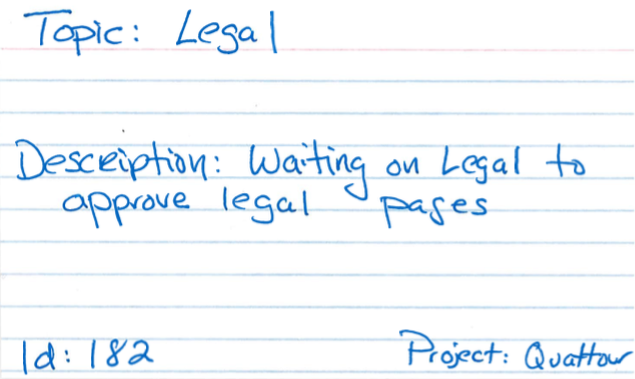
\includegraphics[width=3in]{waste_images/retro_index_card.png}}
\caption{Example Retro Topic Index Card}
\label{exampleRetroTopicl}
\end{figure}














\begin{table}[ht]
\centering
\begin{tabular}{|lll|}
\hline
\multicolumn{3}{|l|}{}  \\
\multicolumn{3}{|l|}{Waste Category: Psychological Distress}  \\
     & \multicolumn{2}{l|}{Cause Property: Low team morale} \\
     &      & Retro Topic: Frustrated developers       \\
     &      & Retro Topic: Not managing expectations       \\
     &      & Retro Topic: Negative attitudes                \\
     &      & Retro Topic: Apathy                            \\
     &      & Retro Topic: Not knowing everyone on the team \\
     &      & Retro Topic: Project feels like it is falling apart emotionally \\
     &      & Retro Topic: Unacknowledged by management      \\
     &      & Retro Topic: Messy code decreasing sense of ownership                    \\
     & \multicolumn{2}{l|}{Cause Property: Rush mode} \\
     &      & Retro Topic: Fixed set of features with a fixed timeline \\
     &      & Retro Topic: Aggressive timelines \\
     &      & Retro Topic: Shifting deadline \\
     &      & Retro Topic: Scope creep \\
     &      & Retro Topic: Repeatedly hearing \quotes{This is due today} \\
     &      & Retro Topic: Long days \\
     &      & Retro Topic: Overtime \\
     & \multicolumn{2}{l|}{Cause Property: Interpersonal or team conflict} \\
     &      & Retro Topic: Criticizing in public \\
     &      & Retro Topic: Difficult pairings \\
     &      & Retro Topic: Pairing fatigue                   \\
     &      & Retro Topic: Not listening \\
     &      & Retro Topic: Interpersonal conflict \\
\multicolumn{3}{|l|}{}  \\
\hline
\end{tabular}
\captionof{figure}{Waste Organization Example (Psychological Distress)}
\label{ChainOfEvidence}
\end{table}



\section{Results: Types of Waste in Software Engineering}
\label{SEWaste}

\begin{table*}[t]
\renewcommand{\arraystretch}{1.3}
\centering
\caption{Types of Software Development Waste}
\label{Waste}
% \begin{tabular}{|p{1.2in}|p{1.9in}|p{3.5in}|} 
\begin{tabular}{|p{1.5in}|p{1.9in}|p{3.2in}|}
% \begin{tabular}{|p{1.7in}|p{1.9in}|p{3in}|} %original draft size
% \begin{tabular}{|p{1.5in}|p{1.6in}|p{2.8in}|} %dissertation size
\hline
Waste  & Description & Observed Causes                                                                                                                                                                                                                                                                                                                                                                                                                     \\ \hline
Building the wrong feature or product &  The cost of building a feature or product that does not address user or business needs. & 
User desiderata (not doing user research, validation, or testing; ignoring user feedback; working on low user value features) \newline 
Business desiderata (not involving a business stakeholder; slow stakeholder feedback; unclear product priorities)                                                                                                                                                                                  \\ \hline
Mismanaging the backlog     & The cost of duplicating work, expediting lower value user features, or delaying necessary bug fixes.  & 
Backlog inversion \newline Working on too many features simultaneously \newline Duplicated work \newline Not enough ready stories  \newline Imbalance of feature work and bug fixing \newline Delaying testing or critical bug fixing \newline Capricious thrashing                                                                                                                                                                                                                                                                                                                                    \\ \hline
Rework                                & The cost of altering delivered work that should have been done correctly but was not. & 
Technical debt \newline
Rejected stories (e.g. product manager rejects story implementation) \newline 
No clear definition of done (ambiguous stories; second guessing design mocks) \newline Defects (poor testing strategy; no root-cause analysis on bugs)                                                                                                                                                                   \\ \hline
Unnecessarily complex solutions  & The cost of creating a more complicated solution than necessary,  a missed opportunity to simplify features, user interface, or code.      & 
Unnecessary feature complexity from the user's perspective \newline
Unnecessary technical complexity (duplicating code, lack of interaction design reuse, overly complex technical design created up-front)
\\ \hline
Extraneous cognitive load &  The costs of unneeded expenditure of mental energy.  &  
Suffering from technical debt \newline	
Complex or large stories \newline	
Inefficient tools and problematic APIs, libraries, and frameworks \newline	
Unnecessary context switching \newline	
Inefficient development flow \newline	
Poorly organized code	
\\ \hline
Psychological distress & The costs of burdening the team with unhelpful stress. &  
Low team morale \newline
Rush mode \newline
Interpersonal or team conflict
\\ \hline
Waiting/multitasking                             & The cost of idle time, often hidden by multi-tasking. & Slow tests or unreliable tests \newline Unreliable acceptance environment \newline Missing information, people, or equipment \newline
Context switching from delayed feedback                                                                                                                                                                                                                                                                          \\ \hline
Knowledge loss & The cost of re-acquiring information that the team once knew. & 
Team churn \newline
Knowledge silos 
\\ \hline
Ineffective communication             & The cost of incomplete, incorrect, misleading, inefficient, or absent communication.                         & 
Team size is too large \newline Asynchronous communication (distributed teams; distributed stakeholders; dependency on another team; opaque processes outside team) \newline Imbalance (dominating the conversation; not listening) \newline Inefficient meetings (lack of focus; skipping retros; not discussing blockers each day; meetings running over (e.g. long stand-ups)) \\ \hline                  
\end{tabular}
\end{table*}




We identified \numberOfWastes{} types of waste (Table \ref{Waste}). This section defines, elaborates, and provides examples of each type, including associated tensions where available.
\subsection{Waste: Building the Wrong Feature or Product}
Building features (or worse, whole products) that no one needs, wants, or uses obviously wastes the time and efforts of everyone involved. We observed this waste affecting team morale, team code ownership \cite{SedanoTeamCodeOwnership}, and customer satisfaction. 

The product features for Project Ses were designed based on a given persona\textemdash i.e. a fictional, archetypal user \cite{Grudin2002personas}. However, consulting several real intended users revealed that the persona was deeply flawed as the users did not need the product. The intended users invalidated the persona. Building the intended product is risky and probably wasteful. 

\textbf{Tension: User needs} versus \textbf{business wants.}
Some projects exhibit a tension between user needs and business goals. Practitioners may struggle to produce something that simultaneously satisfies the users and the business.

On Project Quattuor, the client wanted to add a news feed to a mobile phone application that controlled a real world product in order to increase marketing awareness. However, user validation revealed that no users wanted this feature, and several reacted quite negatively. Despite numerous conversations, the marketing department insisted on adding the feature. 
\subsection{Waste: Mismanaging the Backlog}
The product backlog can be mismanaged in several ways, leading to delays of key features or lower team productivity. 

On several projects, we observed engineers working on low-priority stories through \quotes{backlog inversion.} This occurs when the engineers working through the backlog get ahead of the product manager who is prioritizing the backlog. For instance, the product manager might prioritize the next ten stories in the backlog, but the engineers get to story 15 before the product manager gets back to prioritizing. This creates waste as engineers implement potentially outdated, low-value, or even counterproductive stories ahead of high-value stories.   

Mismanaging the backlog can also lead to duplicated work. We observed duplicate stories in the backlog, two engineers working on the same story because one had forgotten to change its status, and two engineers independently addressing the same pain point (e.g. making the build faster) by not communicating what they were doing in the backlog.

\textbf{Tension: Writing enough stories} versus \textbf{writing stories that will never be implemented.}
Pivotal product managers attempt to provide the team with a steady stream of ready, high-value work. This creates a tension between writing enough stories for the team to work on and \quotes{over-producing} stories that might never be implemented. Writing too few stories causes the team to idle while writing too many stories wastes the product manager's time. We observed teams running out of work on rare occasions; we did not observe product managers writing too many stories.  

\textbf{Tension: Finishing features} versus \textbf{working on too many features simultaneously.}
Product managers decompose a feature into a set of stories and typically aim to create the minimal viable product as quickly as possible by sequencing the stories to finish just enough of each feature before starting another feature. 

On Project Quattuor's backend system, we observed one product manager starting too many tracks of work at once by prioritizing a breadth of features instead of finishing started features. Unfortunately, several tracks of work were not completed by the first release date. The work in progress was disabled with feature flags. Starting work, changing priorities, and halting work in flight can result in waste.

We observed that teams usually prefer to maintain a shippable product while rapidly finishing the simplest possible version of each new feature.

\textbf{Tension: intransigence} versus \textbf{capricious adjustments.}
Responding to change quickly is a core tenet of agile development and often thought of as the opposite of refusing to change. However, responding to change is more like a middle ground between intransigence (unreasonably refusing to change) and thrashing (changing features too often, especially arbitrarily alternating between equally good alternatives). 

On Project Kvin, for example, the launch was delayed while the business fiddled with the sequence and number of steps in the user registration process. Project Duo was similarly delayed by a product manager repeatedly resequencing an order customization process. 
\subsection{Waste: Rework}
From a Waterfall perspective, one might classify any revision of existing code as \quotes{rework.} This problematically fails to distinguish between situations where things could have been done right based on the information available then from situations where new information reveals a better approach. 

Contrastingly, our participants classify revising work that should have been done correctly but was not as \textit{rework}, and improving existing work based on new information as \textit{new work}. \textit{Rework} wastes time and resources by definition. We observed numerous sources of \textit{rework} including technical debt, defects in work products, poor testing strategy, rejected stories, stories with no clear definition of done, and ambiguous mock-ups.
 
Technical debt refers to the risks of delaying needed technical work, by taking technical shortcuts, usually to meet a deadline \cite{McConnellTechnicalDebt}. These shortcuts are waste and often burdens the team later, as described in the \textit{extraneous cognitive load} waste. On Project Quattuor, engineers felt pressured to deliver stories quickly and skipped refactoring, resulting in many weeks of \textit{rework} after the first release. 

Defects and bugs in the code, stories, mock-ups, and code result in \textit{rework}. On every project, we observed defects. On several occasions, mistakes in stories and acceptance criteria resulted in engineering \textit{rework}. On Project Quattuor, the interaction designers created mockups optimized for English, not the target language. After implementing the application, the team realized that the target language text needed more space than the English translations, requiring \textit{rework} for several design components. On Project Kvin, the interaction designer forgot to consider mobile phones when creating the mock-ups. After building a few screens, the team realized that the website did not work well on mobile devices requiring \textit{rework}.

%Poor testing strategy can lead to additional \textit{rework.} On Project Quattuor, the client delayed fixing of critical bugs until just before the release. Fixing one bug in the backend system had a cascading effect on the mobile applications, which expected the code to work a certain way. The team could have avoided \textit{rework} by fixing the critical bug prior to the client code becoming dependent on it.

Rejected stories---stories that a product manager rejects delivered work because the implementation does not satisfy the acceptance criteria---requires \textit{rework} as the developers need to fix the delivered work.

Stories with no clear definition of done (e.g. stories with ambiguous acceptance criteria or ambiguous mock-ups) resulted in \textit{rework}. On Project Ses, the engineers showed a finished story to the interaction designer for feedback. The interaction designer pointed out a missing interaction, which was neither in the story nor the mock-up

\subsection{Waste: Unnecessarily Complex Solutions}
\textit{Unnecessarily complex solutions} can be caused by feature complexity, technical complexity, or lack of reuse. Unnecessary feature complexity wastes users' time as they struggle to understand how to use the system and achieve their objectives, e.g. requiring the user to fill in form fields not related to the task at hand. Some features bring unnecessary technical complexity since a simpler interaction design would have solved the same problem. %\sout{We observed a simple solution was to increase conversations with product, design, and engineering. On one project, an engineer shortened the feedback loop by daily checking-in with the interaction designer.} Unnecessary technical complexity similarly wastes developers' time by making code more difficult to build and maintain. 

On Projects Tes, Ses, and Septem, complicated legacy components were refactored into simpler, easier to understand components. However, personal and organizational goals may misalign on this issue---one Pivotal engineer complained that a client engineer's attitude was, \participantQuote{the more complicated, the better, as that means my role is more important} \textemdash Participant 29.

Another way to increase system complexity is through a lack of reuse, i.e., building a new component instead of reusing an existing one. In code, lack of reuse can manifest as duplicated code and similar components that have similar functionality. In mockups, lack of reuse produces \quotes{snowflake designs,} interaction designs which do not take advantage of design reuse, e.g. two unique user interaction flows that could be unified into similar experiences or two visual components that solve the same concern.

On Project Duo, the interaction designer created a left-to-right navigational flow for configuring the product but designed a top-to-bottom navigational flow for the checkout page. Both sequences allowed the user to change a previous choice, jump to the correct page, and invalidate dependent information. In retrospect, using the same interaction design treatment for both would have been faster. 

On Project Quattuor, multiple interaction designers produced different design treatments for the same concept. The product shipped multiple versions of layouts, lists, alerts, and buttons, some with expensive interactions to delight users. 

On Project Kvin, the interaction designer created two sets of form inputs which necessitated multiple CSS styles for the HTML form input tags. Singular designs require engineering to build unique solutions with no possibility of reuse.   

\textbf{Tension: Big design up-front} versus \textbf{incremental design.}
Many projects exhibit a tension between up-front and incremental design. Rushing into implementation can produce ineffective emergent designs, leading to rework. However, big up-front design can produce incorrect or out-of-date assumptions and inability to cope with rapidly changing circumstances, also leading to expensive rework. The desire to avoid rework and differing development ideologies, therefore, motivates the tension and disagreement over big design up-front versus incremental design. 

The observed teams expected the product features to change even when the client had clearly defined the project. On all projects with interaction designers, after the interaction designer conducted user research and discovered new information about the user's needs, the feature set changed. No amount of up-front consideration appears sufficient to predict user feedback. The observed teams preferred to incrementally deliver functionality and delay integrating with technologies until a feature required it. For example, an engineer would only add asynchronous background jobs technology when working on the first story that requires the needed technology, even if the team knew it would need the technology at the project's beginning.

We observed teams using common architectural and design solutions from similar, previous projects without explicit architectural or design phases.

\subsection{Waste: Extraneous Cognitive Load}

Cognitive Load Theory \cite{Sweller1988} posits that our working memory is quite limited and overloading it inhibits learning and problem solving \cite{Artino2008}. Intrinsic cognitive load refers to the innate complexity of the task, while extraneous cognitive load refers to the cognitive load unnecessarily added by the task environment, or the way the task is presented \cite{Sweller2010}. Reducing the burden on working memory by removing extraneous cognitive load is therefore associated with more efficient learning among other positive outcomes \cite{VanSweller2005}.

Since many software development activities have high intrinsic cognitive load and developer's mental capacity is a limited resource, we view extraneous cognitive load as waste. While we cannot observe cognitive load directly, we did observe sources of extraneous cognitive load including overcomplicated stories, ineffective tooling, technical debt, and multitasking.

Overcomplicated stories---user stories that are unnecessarily long, complex, unclear, or replete with pointers to other necessary information---are precisely the sort of task materials that Cognitive Load Theory predicts will overburden working memory.  On Project Quattuor, one story modifying the presentation of status resulted in the pair creating a spreadsheet listing out the complex behavior. The logic had become too complex to reason about in an individual's working memory. The team, concerned about code maintenance and readability, asked the product manager if simplifying the logic was possible.

Ineffective tooling includes convoluted, nonfunctional, premature, complicated, unstable, outdated, unsupported, time-consuming, or inappropriate-for-the-task software libraries, as well as poorly designed development environments and deployment processes. Participant 13 said that one arcane technology \participantQuote{makes me angry enough that I want to hack into it, expose how useless and horrible it is, and wipe this miserable product off the face of the earth!}

Technical debt introduces the risks of the  code being harder to understand and modify. We observed teams suffering from technical debt with long-running, existing code bases. On Project Tes, for example, running the test suite produced 87,000 lines of output, including deprecation warnings, exceptions, and test noise. Engineers ignored the overwhelming output which contained important information. On Project Ses, dead code littered the code base along with convoluted objects. Project Septem suffered from engineers introducing an idea in one part of the code base, but not applying the concept systematically. These examples illustrate how technical debt creates more things developers need to remember: in other words, how technical debt increases extraneous cognitive load. 

Multitasking---performing two or more activities simultaneously or rapidly alternating between them---increases cognitive load as the multitasker attempts to hold two or more sets of information in working memory or needs to unnecessarily re-load the information into working memory. While observed engineers prefer to finish one task before beginning the next task, they also try to convert excessive waiting (e.g. long builds, long tests, waiting for feedback) into productive time by multitasking (see \textit{waiting/multitasking} waste description for more detail).

\subsection{Waste: Psychological Distress}
\quotes{Stress is the nonspecific response of the body to any demand made upon it} \cite{Selye1976}. Stress may be beneficial (eustress) or harmful (distress). We see psychological distress as a kind of waste for the same reason as \textit{extraneous cognitive load}: developers are a limited resource, which distress consumes. Job-related psychological distress causes absenteeism, burnout, lower productivity, and a variety of health problems \cite{Westman2001}.   
 
On Project Quattuor, for example, the team rushed to release a fixed feature set by a fixed date. Daily, the team decreased a countdown written on an office whiteboard to the release date. We observed low team morale, rush mode, lack of empathy, and waiting too long to resolve interpersonal issues leading to people working inefficiently. Furthermore, the team felt that over-emphasizing the deadline was increasing stress and leading to poor technical decisions and eventually erased the countdown from the whiteboard. Participants felt that fixing both scope and schedule was antithetical to Pivotal's software process, where the client either chooses the release date and gets only the features ready by then or chooses key features and ships the product when the features are ready. 

\subsection{Waste: Waiting/multitasking}
Having developers waiting around, working slowly, or working on low-priority features because something is preventing them from proceeding on high-priority features wastes their time and delays their projects. For example, we observed developers waiting on (or looking for) product managers and designers to clarify a story's acceptance criteria. On Project Quattuor, product managers started multitasking while accepting stories because the acceptance environment was unreliable. We also saw team members waiting around because of missing video-conferencing equipment. 

Ohno described \textit{waiting} waste as hidden waste since people start working on the next job instead of waiting \cite{OhnoToyotaProductionSystem}. The Toyota Production system exposes \textit{waiting} waste by requiring someone to pull the red cable to halt the production line. On Project Ses, it took 58 minutes to run the build locally and 17 minutes on the build machine due to parallelization on four machines. Team members would push code as a branch to the build machine instead of running tests locally. While the build machine ran the tests, the engineers would either wait or context switch onto different work. If the branch passed, some time later, they would merge their code into the team's code. If the branch failed, the engineers would decide either to finish the work that they were doing or to switch back and fix the issue. Some engineers found the context switching exhausting. This \quotes{solution} to avoid \textit{waiting} created \textit{extraneous cognitive load} waste.

\textbf{Tension: Wait, block, or guess.}
When needed information is missing, engineers appear to have three options: 1) wait for the information, 2) suspend (block) the story and work on something else, or 3) act without the information. The best option depends on how far into the story the pair is, how long they have to wait, and their confidence in their guess.

\textbf{Tension: Waiting} versus \textbf{context switching.}
When possible, engineers would often use waiting time to attempt to remedy problems or reduce the duration of future waiting (e.g. shorten the build). When this was not possible, engineers often worked on something else instead of idling. Unfortunately, task switching decreases productivity and increases mistakes \cite{MonsellTaskSwitching}. For short waits, taking a break (e.g. playing table tennis) may be less wasteful than switching to another task. 

\subsection{Waste: Knowledge Loss}
\textit{Knowledge loss} occurs when a team member with unique knowledge leaves a team or company---the latter being a more extreme form of \textit{knowledge loss.}

In projects with knowledge silos, team churn leads to wasted effort as the team regains lost knowledge. For legacy systems, we observed teams sleuthing the code base, commit messages, and completed stories in the backlog to understand the code.  

On Project Octo, a complete team turnover required the new team to spend months understanding the system, during which the team's velocity was practically zero.

The observed teams reduced knowledge loss by actively removing knowledge silos and caretaking the code by adopting the principles, policies, and practices of Sustainable Software Development \cite{SedanoSustainableSoftware}. Teams promoting knowledge sharing appear less susceptible to knowledge loss from team churn or team member rotation. 

\subsection{Waste: Ineffective Communication}
\textit{Ineffective communication} is incomplete, incorrect, misleading, inefficient, or absent communication. We observed that large team sizes, asynchronous communication, imbalance in communication, and inefficient meetings reduced team productivity.

We observed issues with asynchronous communication on Project Quattuor. The team was distributed between two offices separated by an hour commute. We observed the team using remote pairing and engineers commuting between the offices to mitigate the effects of a large distributed team, but communication issues continually arose in the retrospections.

On Project Ses, we observed that one person dominated meetings, which prevented quieter personalities from sharing their perspectives. 

On Project Quattuor, when the project started, the iOS team was not effectively reflecting on its process to make informed decisions. Adding weekly retros helped the team reflect and respond to problems. Over several weeks, the remaining teams added their own retros. 



%When teams are not co-located, additional time is spent on asynchronous communication. Instead of dialoguing about an issue, time is spent crafting a message, sending it, waiting for a response, and interpreting the response. When the message is misunderstood, resolving it takes longer than synchronous communication. When the team is distributed, it loses the benefits of osmotic communication.

%Increasing team size increases the number of communication paths. The number of paths is N x (N -1) / 2. 


% On Project Quattuor, \participantQuote{not enough listening in iOS technical meeting} appeared in two retros. 

% \textit{Ineffective communication} is a well studied topic. \cite{LencioniDeathByMeeting, CollaborationExplained, TabakaCollaborationExplained}.



\section{Comparing to Lean Software Development}
\label{LeanSoftwareDevelopmentComparison}

This section compares and contrasts our waste taxonomy (Section \ref{SEWaste}), with Lean Software Development's waste taxonomy \cite{PoppendieckConceptToCash} category by category. 

While several categories are analogous (Table \ref{LeanSoftwareDevelopmentComparisonTable}), we observed four types of waste not found in Lean: \textit{unnecessarily complex solutions,} \textit{extraneous cognitive load,} \textit{psychological distress,} and \textit{ineffective communication} (see Section \ref{SEWaste} for details). Meanwhile, we did not observe Lean Software Development's \textit{handoff} waste type.

% \begin{table}[t]
% \renewcommand{\arraystretch}{1.5}
% \centering
% \caption{Comparison to Lean Software Development Waste}
% \label{LeanSoftwareDevelopmentComparisonTable}
% \begin{tabular}{|p{1.57in}|p{1.57in}|}
% % \begin{tabular}{|l|l|} %dissertation size
% \hline
% Software Development Wastes           & Lean Software Development Wastes \\ \hline
% Building the wrong feature or product & Extra features                            \\ \hline
% Mismanaging the backlog               & Partially done work                            \\ \hline
% Unnecessarily complex solutions                & Not described                             \\ \hline
% Rework                                & Defects                                   \\ \hline
% Extraneous cognitive load                 & Task switching  \\ \hline
% Psychological distress                             & Not described \\ \hline
% Waiting                               & Delays                                    \\ \hline
% Knowledge loss                 & Relearning                            \\ \hline
% Ineffective communication             & Not described                             \\ \hline
% Not observed                          & Handoffs                                  \\ \hline
% \end{tabular}
% \end{table}


\begin{table}[t]
\renewcommand{\arraystretch}{1.5}
\centering
\caption{Comparison to Lean Software Development Waste}
\label{LeanSoftwareDevelopmentComparisonTable}
\begin{tabular}{|p{1.57in}|p{1.57in}|}
% \begin{tabular}{|l|l|} %dissertation size
\hline
Software Development Wastes           & Lean Software Development Wastes \\ \hline
Building the wrong feature or product & Extra features                            \\ \hline
Mismanaging the backlog               & Partially done work                            \\ \hline
Rework                                & Defects                                   \\ \hline
Unnecessarily complex solutions                & Not described                             \\ \hline
Extraneous cognitive load                 & Not described  \\ \hline
Psychological distress                             & Not described \\ \hline
Waiting/multitasking                              & Delays                                    \\  
                  & Task switching  \\ \hline
Knowledge loss                 & Relearning                            \\ \hline
Ineffective communication             & Not described                             \\ \hline
Not observed                          & Handoffs                                  \\ \hline
\end{tabular}
\end{table}




\textbf{Handoffs}: We did not observe \textit{handoff} waste---the loss of tacit knowledge when work is handed off to colleagues---as Pivotal follows an iterative software development process with cross-functional teams. We did observe \textit{waiting} waste as engineers might contact people outside the team who had needed information. \textit{Handoffs} certainly contribute to the wastes of \textit{knowledge loss}, \textit{ineffective communication}, and \textit{waiting}. However, our data does not support \textit{handoffs} as a \textit{type} of waste.

\textbf{Building the wrong feature or product} and \textbf{Extra features}: In our model, \textit{building the wrong feature or product} describes not addressing user or business needs. Pivotal's process relies on user validation to assess value in solving the user's needs and iterating from a minimal viable product. In Lean Software Development, the \textit{extra features} waste describes adding in features that are not necessary for the user's current needs. Both perspectives align on delaying features until necessary. \textit{Extra features} does not cover the waste from missing important business needs. \textit{Building the wrong feature or product} subsumes \textit{extra features}.

\textbf{Mismanaging the backlog} and \textbf{Partially done work}: There is common ground between both taxonomies on reducing large batch sizes into smaller batches with an ideal of  \quotes{continuous flow,} where work is routinely moving through the system hence decreasing feature lead time. However, in Lean Software Development, \textit{partially done work} is work that is not tested, implemented, integrated, documented, or deployed. Any feature description that is not implemented, any code that is not integrated or merged, any code that is untested, any code that is not self-documenting or documented, and any code that is not deployed where the user can receive value is \textit{partially done work}.

The observed teams did not view materials flowing through the system as waste. Interaction designers need to produce just enough mockups, product managers need to write just enough stories, and developers need to write just enough code to make the story work. In any continuous flow system, there are unfinished materials at each step. 

While we did observe a product manager starting too many features at once (as described in the \textit{mismanaging the backlog} waste section), we mostly observed work flowing in a relatively orderly fashion with minimal delay. Large amounts of waiting designs or stories would have been classified as \textit{mismanaging the backlog} waste.

\textit{Mismanaging the backlog} includes observed wastes beyond \textit{partially done work}, namely,  sequencing low priority work before high priority work, accidentally duplicating work, capricious thrashing, or delaying necessary bug fixes. Lean Software Development does not cover these wastes. 

%Just-in-time production is antithetical to large batch sizes. In any continuous flow system, there is unfinished materials at each step. 

%Based on this understanding of continuous flow, we believe that \textit{\partially done work} is suggesting that large batch sizes need reducing.   

%The Toyota Production System creates buffers of parts at certain steps in the pipeline, like a bumper sits waiting to be used on the next car. Once that bumper is consumed, the process of creating another bumper just like it is started. Enough material is produced to keep continuous flow moving. Ohno was concerned about the stockpiles of inventory stored in warehouses.

%Since Pivotal engineers follow Test Driven Development / Behavior Driven Development, strive to get the tested code into the developer's master branch as quickly as possible, and release frequently, we did not observe the waste associated with partially done work. At any moment in time, an interaction designer is creating a future mock, a product manager is updating a future story, a developer is testing code that has not shipped. This describes the continuous flow of features to the customer. 

\textbf{Rework} and \textbf{Defects}: While both taxonomies agree on \textit{defects} as waste, our \textit{rework} concept subsumes \textit{defects}. \textit{Rework} includes mistakes made by the product managers (in writing acceptance criteria), the interaction designers (in creating mockups) and the developers (in writing tests and code). Poor testing strategies and delaying testing can cause rework. \textit{Rework} also includes shortcuts intentionally made by team members to save time leading to technical debt. Finally, our definition of \textit{rework} distinguishes mistakes that could have been avoided from problems only obvious in hindsight. 

\textbf{Waiting/multitasking} and \textbf{Task switching}: \textit{Multitasking} and \textit{task switching} describe the same behavior. The desire to have developers work on one thing at a time is common to both models. 

\textbf{Waiting/multitasking} and \textbf{Delays}: In our model, \textit{waiting} includes delays from not having the needed information or resources to get one's work done as well as the cost of slow tests and unreliable tests. In Lean Software Development, \textit{delays} are \quotes{waiting for people to be available who are working in other areas} to provide needed information that is not available to the developers \cite{PoppendieckConceptToCash}. Both wastes describe the cost of missing needing information. \textit{Waiting} subsumes \textit{delays}.

\textbf{Knowledge loss} and \textbf{Relearning}:
In our model, \textit{knowledge loss} is the cost from members rolling off the team. In Lean Software Development, \textit{relearning} is \quotes{rediscovering something we once knew} \cite{PoppendieckConceptToCash}, which includes the cost of an individual not remembering a decision already made. The observed teams see forgetting as a natural part of the human experience, not as a waste.  Included in \textit{relearning} is failing to engage people in the development process. We did observe product managers having difficulty in involving some stakeholders, which we include in the \textit{building the wrong feature or product} waste. \textit{Knowledge loss} focuses \textit{relearning} to simply regaining departed knowledge. 
\section{Results Evaluation and Quality Criteria}
\label{ResultsEvaluation}
While other factors may affect software engineering waste, we focus only on those that we observed during the study. Grounded Theory studies can be evaluated using the following criteria \cite{Charmaz, StolGroundedTheory}:

\textbf{Credibility}: \quotes{Is there sufficient data to merit claims?}  This study relies on \durationOfResearchStudyPlural{} of participant-observation, \numberOfInterviews{} intensive open-ended interviews, and one year's worth of retrospections. 

\textbf{Originality}: \quotes{Do the categories offer new insights?}  This study is the first empirical study of waste in software development. It not only discovered new waste types but also supports and expands existing waste types that have not previously undergone rigorous empirical validation in a software engineering context. 

\textbf{Resonance}: \quotes{Does the theory make sense to participants?} We presented the results to the organization. Seven participants reviewed the results and this paper. They indicated that the waste taxonomy resonates with their experience: \quotes{These are pain points that we all felt. This covers what we learned on the projects} \textemdash Participant 33; \quotes{I have lived through these projects\ldots No other waste comes to mind} \textemdash Participant 31. This process produced no significant changes, which is not surprising because participant observation mitigates resonance problems.

\textbf{Usefulness}: \quotes{Does the theory offer useful interpretations?} This study identifies software development wastes that are not identified in manufacturing and explains why certain behaviors, events, and actions can cause software engineering waste. It provides a rich waste taxonomy for identifying wastes in practice. %and for Value Stream Mapping. 

Regarding \textbf{external validity}, Grounded Theory is non-statistical, non-sampling research; therefore, the results cannot be statistically generalized to a population. Based on existing research and our experience, none of the identified wastes appear peculiar to Pivotal or Extreme Programming. However, Pivotal is a very effective organization, which uses iterative development and has been concerned with eliminating waste for almost two decades. Organizations that are newer, less experienced, less concerned with waste, or use less iterative methods may experience additional waste types. For example, \textit{waiting} waste manifests in organizations that hand feature documents between teams or use large batch sizes of features \cite{Ali2016, Khurum2014, Mujtaba2010}. Researchers and professionals should, therefore, take care to adapt our findings to their contexts case-by-case. 

Finally, the results might be influenced by \textbf{researcher bias} or \textbf{prior knowledge bias}. During participant observation, the researcher may lose perspective and become biased by being a member of the team. That is, while a participant-observer gains perspective an outsider cannot, an outside observer might see something a participant observer will miss. Similarly, while prior knowledge helps the researcher interpret events and select lines of inquiry, prior knowledge may also blind the researcher to alternative explanations \cite{GlaserIssues}. We mitigated these risks by recording interviews and having the second and third authors review the coding process.
\section{Conclusion}
\label{Conclusion}
This paper presents the first evidence-based taxonomy of software engineering waste, identifies numerous causes of waste, and explores fundamental tensions related to specific waste types. \numberOfWastesCapitalized{} waste types are identified: building the wrong feature or product, mismanaging the backlog, rework, unnecessarily complex solutions, extraneous cognitive load, 
psychological distress, waiting/multitasking, knowledge loss, and ineffective communication. Each waste is illustrated with examples taken from observed projects at Pivotal, showing how the waste materializes, and in some cases how it is removed or eliminated. We also compare our taxonomy to Lean Software Development's waste taxonomy.

Our taxonomy emerged from a Constructivist Grounded Theory study, including the collection and analysis of data from \durationOfResearchStudyPlural{} of participant-observation of  \numberOfObservedProjects{} software development projects; interviews of \numberOfInterviews{} software engineers, interaction designers, and product managers; as well as one year of retrospection topics. The analysis of the retrospection topics reveals that the observed Pivotal teams care deeply about finding and eliminating waste in their software development processes. 

While this research supports parts of the Lean Software Development waste taxonomy, it differs in three key ways: 1) it introduces four new waste categories: \textit{unnecessarily complex solutions,} \textit{extraneous cognitive load,} \textit{psychological distress,} and \textit{ineffective communication}; 2) it does not support Lean Software Development's \textit{handoffs} waste category; and 3) its waste categories are largely broader than Lean Software Development's categories. As such, our taxonomy is more expressive and more accurately describes the observed data. To be clear, the Lean Software Development's taxonomy of wastes was developed top-down, by mapping manufacturing wastes onto software development concepts. It was not empirically tested and therefore does not have the same epistemic status as our taxonomy, which was developed bottom-up from rigorous primary data collection and analysis. 

Several avenues for future research have potential. Studying different kinds of projects in different organizations may reveal new types of waste, or improve our understanding of existing categories. Furthermore, understanding wastes and their causes is just the first step in devising techniques for reducing waste and mitigating its effects. We would also like to investigate how teams use feedback loops to identify, manage, and reduce waste. 

%\sout{At the core of Lean Thinking is waste identification and elimination \cite{WomackLeanThinking} which is a key differentiator between Lean and Agile in software development \cite{Fitzgerald2015continuous}. (Agile does promote the use of feedback loops which we observed as a common solution for waste identification and removal at Pivotal.)

%Ohno and Shingo singularly focused on the efficiency of the production line through continuous waste removal. By excluding product development activities, the design of the vehicle, they overlooked the entire picture. This may explain why their waste taxonomy misses aspects fundamental to product design.

%In applying waste removal to software development, it behooves the software community first to start with a waste taxonomy grounded in data from software development, not borrow from a dissimilar domain. Since waste removal is core to the Lean movement, starting with an ill formulated waste taxonomy suggests a possible fundamental impact on Lean Software Development claims.

%This work suggests that evidence-based research yields insights grounded in data that have not emerged from applying manufacturing concepts to software development.}

%\sout{Based on the research from value stream mapping, the first step of waste reduction may be switching a software firm from a batch-and-pull process where a feature document is handed to a team to implement (e.g. a waterfall system) to a system where a small number of features are handed to a team (e.g. iterative software development.) Then introducing and reducing feedback loops to remove additional waste.}
\section*{Acknowledgement}
Thanks to Ben Christel for his assistance in sorting retro topics and helping with the initial analysis. Thank you to Rob Mee, David Goudreau, Ryan Richard, Zach Larson, Elisabeth Hendrickson, and Michael Schubert for making this research possible.






% \begin{table}[]
% \centering
% \caption{Examples for People working inefficiently waste}
% \label{chainOfEvidence}
% \begin{tabular}{|llll|}
% \hline
% \multicolumn{4}{|l|}{}  \\
% \multicolumn{4}{|l|}{Waste category: People working inefficiently}  \\
%     & \multicolumn{3}{l|}{Cause category: Emotional stress}          \\
%     &     & \multicolumn{2}{l|}{Cause property: Low team morale} \\
%     &     &      & Retro Topic: Frustrated Clients / Pivots       \\
%     &     &      & Retro Topic: Negative attitudes                \\
%     &     &      & Retro Topic: Apathy                            \\
%     &     &      & Retro Topic: Unacknowledged by management      \\
%     &     &      & Retro Topic: Messy code                        \\
%     &     &      & Retro Topic: Pairing fatigue                   \\
%     &     &      & Retro Topic: Poor lighting, lack of windows    \\
%     &     & \multicolumn{2}{l|}{Cause property: Rush mode} \\
%     &     &      & Retro Topic: Fixed features with a fixed timeline \\
%     &     &      & Retro Topic: Aggressive timelines \\
%     &     &      & Retro Topic: Scope creep \\
%     &     &      & Retro Topic: This has to be done today \\
%     &     &      & Retro Topic: Repeatedly saying “This has to be done today” \\
%     &     &      & Retro Topic: Long days \\
%     &     &      & Retro Topic: Overtime \\
%     &     & \multicolumn{2}{l|}{Cause property: Lack of empathy} \\
%     &     &      & Retro Topic: Not listening \\
%     &     &      & Retro Topic: Criticizing in public \\
%     &     &      & Retro Topic: Difficult pairings \\
%     &     &      & Retro Topic: Interpersonal conflict \\
%     &     &      & Retro Topic: Kicking product out of the team space \\
%     &     & \multicolumn{2}{l|}{Cause property: Waiting too long to resolve interpersonal issues} \\
%     & \multicolumn{3}{l|}{Cause category: Cognitive load}          \\
%     &     & \multicolumn{2}{l|}{\dots} \\
%     & \multicolumn{3}{l|}{Cause category: Suffering from Technical debt}          \\
%     &     & \multicolumn{2}{l|}{\dots} \\
%     & \multicolumn{3}{l|}{Cause category: Inefficient tools and libraries}          \\
%     &     & \multicolumn{2}{l|}{\dots} \\
% \hline
% \end{tabular}
% \end{table}

% \begin{table}[]
% \renewcommand{\arraystretch}{1.5}
% \centering
% \caption{Example Retro Topic Index Card }
% \label{exampleRetroTopicl}
% \begin{tabular}{|l|}
% \hline
% Topic: Legal \\ \\ Description: Waiting on Legal to approve legal pages \\ \\ Id: 182 Project: Quattour\\ \hline
% \end{tabular}
% \end{table}


% \begin{table}[t]
% \renewcommand{\arraystretch}{1.5}
% \centering
% \caption{Comparison of Manufacturing Waste with Lean Software Development Waste}
% \label{ManufacturingVersusLeanSoftwareWastel}
% \begin{tabular}{|p{1.57in}|p{1.57in}|}
% \hline
% Toyota Production System’s Manufacturing Wastes & Poppendieck’s Software Development Wastes \\ \hline
% Inventory                                       & Partially Done Work                       \\ \hline
% Extra Processing                                & Relearning                                \\ \hline
% Overproduction                                  & Extra Features                            \\ \hline
% Transportation (of goods)                       & Handoffs                                  \\ \hline
% Waiting                                         & Delays                                    \\ \hline
% Motion (of people)                              & Task Switching                            \\ \hline
% Defects                                         & Defects                                   \\ \hline
% Value (added by Womack in 1996)                 & N/A                                       \\ \hline
% Non-utilized Talent(added by Liker in 2004)     & N/A                                       \\ \hline
% \end{tabular}
% \end{table}
























% \begin{table}[]
% \renewcommand{\arraystretch}{1.5}
% \centering
% \caption{My caption}
% \label{my-label}
% \begin{tabular}{|p{1.3in}|p{2.1in}|}
% \hline
% Waste                                & Observed Causes                                                                                                                                                                                                                                                                                                                                                                                                                                                                 \\ \hline
% Building the wrong feature or product & \begin{tabular}[c]{@{}l@{}}User Desiderata\\ Not doing user research, validation, or testing\\ Ignoring user feedback \\ Working on low user value features\\ \\ Business Desiderata\\ Not involving a stakeholder\\ Slow stakeholder feedback\\ \end{tabular}                                                                                                                                                                                                                                                                      \\ \hline
% Mismanaging the backlog              & \begin{tabular}[c]{@{}l@{}}Backlog inversion\\ Duplicated story\\ Forgetting to start a story \\ Too much work in progress\end{tabular}                                                                                                                                                                                                                                                                                                                                         \\ \hline
% Unnecessary uniqueness or complexity & \begin{tabular}[c]{@{}l@{}}Unnecessary feature complexity\\ Snowflake designs\\ Unnecessary technical complexity\\ Big design up-front\\ Duplicating of code\end{tabular}                                                                                                                                                                                                                                                      \\ \hline
% Rework                               & \begin{tabular}[c]{@{}l@{}}Definition of done not clear\\ Ambiguous story\\ Second guessing design mocks\\ \\ Rejected Stories\\ \\ Defects / Bugs\\ Poor testing strategy\\ Not doing root cause analysis on bugs\\ Delaying testing or critical bug fixing\end{tabular}                                                                                                                                                                                              \\ \hline
% People working inefficiently         & \begin{tabular}[c]{@{}l@{}}Emotional Stress\\ Low team morale\\ Rush mode\\  Lack of empathy\\  \\ Cognitive Load\\ Complex stories\\ Noisy output from tools\\ \\ Inefficient tools and libraries\\ Inefficient tooling \\ Problematic APIs, libraries, and frameworks\end{tabular}                                                                                                    \\ \hline
% Suffering from technical debt        & \begin{tabular}[c]{@{}l@{}}Technical debt\\ Hard to change code\end{tabular}                                                                                                                                                                                                                                                                                                                                                                                                    \\ \hline
% Waiting                              & \begin{tabular}[c]{@{}l@{}}Slow tests or unreliable tests\\ Unreliable acceptance environment\\ Missing product manager\\ Missing equipment\end{tabular}                                                                                                                                                                                                                                                                                                                        \\ \hline
% Unnecessary cognitive effort         & \begin{tabular}[c]{@{}l@{}}Ambiguity\\ Unclear bug reports\\ Messy code \\ Unclear git commit messages\\ \\ \\ Knowledge loss from team churn\\ \\ \\ Context switching due to delayed feedback\\ Context switching\\ PMs taking a long time to accept or reject a story\\ Missing a PM for periods of time\\ Missing a Designer for periods of time\\ Design / Developer pairing not happening\end{tabular} \\ \hline
% Ineffective communication            & \begin{tabular}[c]{@{}l@{}}Too large team size\\ \\ Asynchronous communication\\ Distributed teams\\ Non-collocated stakeholder\\ Dependency on another team\\ Opaque processes outside team\\ \\ Imbalance in communication\\ One person dominating the conversation\\ Not listening\\ \\ Inefficient meetings\\ Lack of focus\\ Teams skipping retros\\ Not discussing blockers each day\\ Meetings running over (e.g. long standups)\end{tabular}      \\ \hline
% Thrashing on features or code        & Disagreement(Lack of transitivity of preference)                                                                                                                                                                                                                                                                                                                                                                                                                                \\ \hline
% \end{tabular}
% \end{table}














% An example of a floating figure using the graphicx package.
% Note that \label must occur AFTER (or within) \caption.
% For figures, \caption should occur after the \includegraphics.
% Note that IEEEtran v1.7 and later has special internal code that
% is designed to preserve the operation of \label within \caption
% even when the captionsoff option is in effect. However, because
% of issues like this, it may be the safest practice to put all your
% \label just after \caption rather than within \caption{}.
%
% Reminder: the "draftcls" or "draftclsnofoot", not "draft", class
% option should be used if it is desired that the figures are to be
% displayed while in draft mode.
%
%\begin{figure}[!t]
%\centering
%\includegraphics[width=2.5in]{myfigure}
% where an .eps filename suffix will be assumed under latex, 
% and a .pdf suffix will be assumed for pdflatex; or what has been declared
% via \DeclareGraphicsExtensions.
%\caption{Simulation Results}
%\label{fig_sim}
%\end{figure}

% Note that IEEE typically puts floats only at the top, even when this
% results in a large percentage of a column being occupied by floats.


% An example of a double column floating figure using two subfigures.
% (The subfig.sty package must be loaded for this to work.)
% The subfigure \label commands are set within each subfloat command, the
% \label for the overall figure must come after \caption.
% \hfil must be used as a separator to get equal spacing.
% The subfigure.sty package works much the same way, except \subfigure is
% used instead of \subfloat.
%
%\begin{figure*}[!t]
%\centerline{\subfloat[Case I]\includegraphics[width=2.5in]{subfigcase1}%
%\label{fig_first_case}}
%\hfil
%\subfloat[Case II]{\includegraphics[width=2.5in]{subfigcase2}%
%\label{fig_second_case}}}
%\caption{Simulation results}
%\label{fig_sim}
%\end{figure*}
%
% Note that often IEEE papers with subfigures do not employ subfigure
% captions (using the optional argument to \subfloat), but instead will
% reference/describe all of them (a), (b), etc., within the main caption.


% An example of a floating table. Note that, for IEEE style tables, the 
% \caption command should come BEFORE the table. Table text will default to
% \footnotesize as IEEE normally uses this smaller font for tables.
% The \label must come after \caption as always.
%
%\begin{table}[!t]
%% increase table row spacing, adjust to taste
%\renewcommand{\arraystretch}{1.3}
% if using array.sty, it might be a good idea to tweak the value of
% \extrarowheight as needed to properly center the text within the cells
%\caption{An Example of a Table}
%\label{table_example}
%\centering
%% Some packages, such as MDW tools, offer better commands for making tables
%% than the plain LaTeX2e tabular which is used here.
%\begin{tabular}{|c||c|}
%\hline
%One & Two\\
%\hline
%Three & Four\\
%\hline
%\end{tabular}
%\end{table}


% Note that IEEE does not put floats in the very first column - or typically
% anywhere on the first page for that matter. Also, in-text middle ("here")
% positioning is not used. Most IEEE journals/conferences use top floats
% exclusively. Note that, LaTeX2e, unlike IEEE journals/conferences, places
% footnotes above bottom floats. This can be corrected via the \fnbelowfloat
% command of the stfloats package.





% trigger a \newpage just before the given reference
% number - used to balance the columns on the last page
% adjust value as needed - may need to be readjusted if
% the document is modified later
%\IEEEtriggeratref{8}
% The "triggered" command can be changed if desired:
%\IEEEtriggercmd{\enlargethispage{-5in}}

% references section

% can use a bibliography generated by BibTeX as a .bbl file
% BibTeX documentation can be easily obtained at:
% http://www.ctan.org/tex-archive/biblio/bibtex/contrib/doc/
% The IEEEtran BibTeX style support page is at:
% http://www.michaelshell.org/tex/ieeetran/bibtex/
%\bibliographystyle{IEEEtran}
% argument is your BibTeX string definitions and bibliography database(s)
%\bibliography{IEEEabrv,../bib/paper}
%
% <OR> manually copy in the resultant .bbl file
% set second argument of \begin to the number of references
% (used to reserve space for the reference number labels box)
% \begin{thebibliography}{1}

% \bibitem{IEEEhowto:kopka}
% H.~Kopka and P.~W. Daly, \emph{A Guide to \LaTeX}, 3rd~ed.\hskip 1em plus
%   0.5em minus 0.4em\relax Harlow, England: Addison-Wesley, 1999.

% \end{thebibliography}
\bibliographystyle{IEEEtran}
% \bibliographystyle{abbrv}
\bibliography{bibliography} 



% that's all folks
\end{document}


